\documentclass[12pt,a4paper,oneside]{report}
\usepackage{graphicx}
\usepackage{german,a4}
%\usepackage{picins}
%\usepackage{epsfig}
\usepackage{lmodern}
\usepackage{fancyhdr}
\usepackage[utf8]{inputenc}
%\usepackage{setspace}
\usepackage[T1]{fontenc}
\usepackage{hyperref}
\usepackage[sf]{titlesec}
\usepackage{textcomp}
\usepackage{makeidx}
\usepackage{amsmath}
%\usepackage[ngerman]{babel}
\usepackage{listings}
\usepackage{color}
\usepackage{colortbl}
\definecolor{lightgray}{rgb}{0.8,0.8,0.8}
\definecolor{darkgreen}{rgb}{0,0.6,0}
\usepackage{pdfpages}
\usepackage{graphicx}
\usepackage{cite}
\usepackage{listings}
\usepackage{array} 
%\usepackage{helvet}
%\usepackage{graphicx}
\usepackage{caption}
\usepackage{subcaption}
\usepackage[font=small,labelfont=bf]{caption}
\usepackage[utf8]{inputenc}
% =====================================================
% Seite einrichten
% =====================================================
\setlength{\textwidth}{160mm} \setlength{\textheight}{235mm}
\setlength{\evensidemargin}{5mm} \setlength{\oddsidemargin}{5mm}
\setlength{\topmargin}{0mm} \setlength{\voffset}{-15mm}
\setlength{\headsep}{12mm} \setlength{\footskip}{15mm}
\setlength{\headheight}{15.1pt}

% =====================================================
% sonstige Einstellungen
% =====================================================
%\flushbottom % Textfluss schoen unten ausrichten
\footnotesep12pt % Abstand Text / Fussnote
%\setlength{\parindent}{0pt} \setlength{\abovecaptionskip}{-6pt}
%\setlength{\belowcaptionskip}{0pt} \setlength{\intextsep}{18pt}
%\renewcommand{\baselinestretch}{1.2} % Zeilenabstand
\setcounter{secnumdepth}{4}
\newcommand{\p}[1]{\texttt{#1}}
\nonfrenchspacing

% =====================================================
% Kopf- und Fusszeile formatieren
% =====================================================
\pagestyle{fancy}
\lhead[LE,RO]{\sf{\leftmark}}
\rhead[RE,LO]{\sf{\thepage}}
\lfoot{\setlength{\unitlength}{1mm}
\begin{picture}(0,0)
\put(0,-2){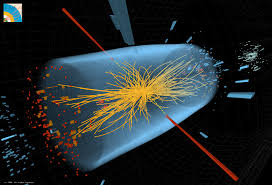
\includegraphics[height=0.6cm,width=0.8cm]{images/ppp.jpg}}
\end{picture}\put(10,2){\scriptsize\sf{Institut for theoretical physics}}\put(10,-2){\scriptsize\sf{Karlsruher institut for Technology (KIT)}}}
\cfoot{}
\rfoot{\footnotesize\sf{Thesis by Tigran Saidnia}}
\renewcommand{\headrulewidth}{0.4pt}
\renewcommand{\footrulewidth}{1.0pt}
\newcommand{\offline}{$ \overline{\textrm{\textbf{Off}}}\underline{\textrm{\textbf{line}}}\ $}


% ====================================================
% Kopf- und Fusszeile fuer "plain"-Format ueberschreiben
% ====================================================
\fancypagestyle{plain}{%
\fancyhf{}
\fancyfoot[L,C,R]{\setlength{\unitlength}{1mm}
\begin{picture}(0,0)
\put(0,-2){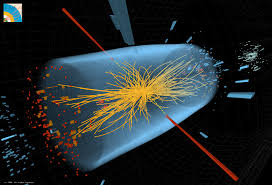
\includegraphics[height=0.6cm,width=0.8cm]{images/ppp.jpg}}
\end{picture}\put(10,2){\scriptsize\sf{Institut for theoretical physics}}\put(10,-2){\scriptsize\sf{Karlsruhe Institut of Technology (KIT)}}}
\cfoot{}
\rfoot{\footnotesize\sf{Thesis by Tigran Saidnia}}
\renewcommand{\headrulewidth}{0pt}
\renewcommand{\footrulewidth}{1.0pt}}

\begin{document}

%\doublespacing
    \parindent=0pt
    %\sloppypar
    \linespread{1.2}
    \thispagestyle{plain}
    %\frontmatter
    %\maketitle


\begin{titlepage}

\begin{center}


% Oberer Teil der Titelseite:

\includegraphics[width=0.3\textwidth]{images/Intro/kitlogo_de_rgb}\\[1cm]    

\textsc{\LARGE Master Thesis}\\[0.5cm]
\textsc{\Large by}\\[0.5cm]
\textsc{\Large Tigran Saidnia}\\[1.0cm]


% Title
\newcommand{\HRule}{\rule{\linewidth}{0.5mm}}
\HRule \\[0.8mm]
{\textbf{\Large \bfseries Emission kernels of parton showers in LO}}\\[0.8mm]

%\HRule \\[0.001mm]
%\newcommand{\HRule}{\rule{\linewidth}{0.5mm}}
%\HRule \\[0.8mm]
%{\textbf{\bfseries Emission kernels of parton showers in LO}}\\[0.8mm]

\HRule \\[1cm]
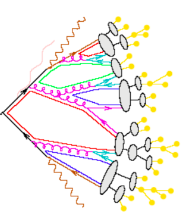
\includegraphics[scale=0.7]{images/Intro/footPicture.PNG}\\[0.8cm]   

\Large Karlsruhe institute of Technology (KIT)\\[1.5mm]
\Large Institute for theoretical physics\\[1.0cm]

{\Large Reviewer: PD Dr. Stefan Gieseke \\
\Large Second reviewer: Prof. Dr. Dieter Zeppenfeld\\
\Large External advisor: Dr. Simon Plätzer\\
\Large Advisor: Emma Simpson Dore}\\[0.8cm]   

Duration: July 1, 2018  –  July 1, 2019

\vfill

% Unterer Teil der Seite
 %\today

\end{center}

\end{titlepage}

\pagebreak

\thispagestyle{empty}
\quad
\newpage
%\input{zusammenfassung}
\chapter*{}
\begin{flushleft}
\vspace{11cm}
\textbf{Statement of Originality}\\[1cm]
I hereby confirm that I have written the accompanying thesis by myself, without contributions from any sources other than those cited in the text and acknowledgements. This applies also to all graphics, drawings, maps and images included in the thesis.\\[1cm]

Karlsruhe, \today \\[1cm]
\end{flushleft}

\begin{center}
---------------------------------\\
Tigran Saidnia
\end{center}

\pagebreak

\thispagestyle{empty}
\quad
\newpage
\pagenumbering{Roman}


\input{abstract/abtract.tex}
\pagebreak

\thispagestyle{empty}
\quad
\newpage

  
    \tableofcontents
    \thispagestyle{empty}
    
        \pagebreak
        \clearpage
        \pagenumbering{arabic} 

\thispagestyle{empty}
\quad
\newpage
   
\setcounter{page}{1}

   

    \newpage 
\thispagestyle{empty}
\quad 
\newpage
   

    \addcontentsline{toc}{chapter}{Literaturverzeichnis}
    \bibliographystyle{plain}
    \bibliography{bibliography2}

    %\listoftables
    %\listoffigures
    %\printindex

    \appendix
        \newpage 
\thispagestyle{empty}
\quad 
\newpage
   
First of all I would like to thank all those who supported me during the preparation of this work and who contributed a lot to the success of this work, in particular:\\
\\
PD Dr. Stefan Gieseke for his excellent care and patience.\\
\\
Prof. Dr. Dieter Zeppenfeld for the takeover of the second assessor.\\
\\
Dr. Simon Plätzer who gave me a helpful feedback and took the time to discuss this work.\\
My great thanks also go to Emma Simpson Dore, who proofread my work in numerous hours. She pointed out to me the weaknesses of my letter and showed me the right paths to reach my goal at work.\\
\\ 
Finally, I would like to thank my girlfriend Canan Kaman, who supported me in all things in this not always easy time.\\


 
         


 


   % \chapter{Quellcode}

\lstset{language=vhdl, basicstyle=\ttfamily\footnotesize, keywordstyle=\color{blue}, commentstyle=\color{darkgreen}, breaklines=true, frame=none, numberbychapter=false, captionpos=b, caption={}}

Deaktiviertes Fetch-Pipeline-Register, modifiziertes Decode-Pipeline-Register

\begin{lstlisting}
--  type fetch_reg_type is record
--    pc     : pctype;
--    branch : std_ulogic;
--  end record;
  
  type decode_reg_type is record
    pc, branch_next_address    : pctype;
    branch, branch_next : std_ulogic;
    inst  : icdtype;
    cwp   : cwptype;
    set   : std_logic_vector(ISETMSB downto 0);
    mexc  : std_ulogic;
    cnt   : std_logic_vector(1 downto 0);
    pv    : std_ulogic;
    annul : std_ulogic;
    inull : std_ulogic;
    step  : std_ulogic;        
    divrdy: std_ulogic;        
  end record;
\end{lstlisting}

Funktionalität von Instruction Fetch, übertragen an Decode:

\begin{lstlisting}

    bpmiss := ex_bpmiss or ra_bpmiss;
    npc := r.d.pc; de_pc := r.d.pc;
    if ra_bpmiss = '1' then de_pc := r.d.pc; end if;
    if ex_bpmiss = '1' then de_pc := r.e.ctrl.pc; end if;
    de_npc := zero32(31 downto PCLOW);
    de_npc(31 downto 2) := de_pc(31 downto 2) + 1;    -- Address incrementer

    if (xc_rstn = '0') then
      v.d.pc := (others => '0'); v.d.branch := '0';
      if DYNRST then v.d.pc(31 downto 12) := irqi.rstvec;
      else
        v.d.pc(31 downto 12) := conv_std_logic_vector(rstaddr, 20);
      end if;
    elsif xc_exception = '1' then	-- exception
      v.d.branch := '1';
      v.d.branch_next := '1'; v.d.branch_next_address := xc_trap_address;
      if ( r.d.branch_next = '1' ) then
      	v.d.pc := r.d.branch_next_address; npc := v.d.pc;
      else
      v.d.pc := de_npc;
      npc := v.d.pc;
      end if;
    elsif de_hold_pc = '1' then
      v.d.pc := r.d.pc; npc := v.d.pc; v.d.branch := r.d.branch; v.d.branch_next := r.d.branch_next;
      if bpmiss = '1' then
        v.d.pc := de_npc ; v.d.branch := '1'; v.d.branch_next := '0';
        npc := v.d.pc;
      elsif ex_jump = '1' then
        v.d.branch_next := '1'; v.d.branch_next_address := ex_jump_address ;
        v.d.pc := de_npc; v.d.branch := '1';
        npc := v.d.pc ;
      end if;    
    elsif (ex_jump and not bpmiss) = '1' then
      v.d.branch_next := '1'; v.d.branch_next_address := ex_jump_address ;
      if r.d.branch_next = '1' then
      	v.d.pc := r.d.branch_next_address;
      else
      v.d.pc := de_npc; end if; 
      v.d.branch := '1'; npc := v.d.pc ;
    elsif (de_branch and not bpmiss) = '1' then
      if jump_next = '1' then
        if de_inst(28 downto 25) = BA then
          v.d.branch_next := '1'; v.d.branch_next_address := branch_address(de_inst, r.d.pc); npc := v.d.pc; v.d.branch := '1';
          --v.d.pc:= de_npc + '1'; npc := v.d.pc; v.d.branch := '1'	;
        else
          v.d.pc := de_npc + '1'; npc := v.d.pc; v.d.branch := '1';
          v.d.branch_next := '1'; v.d.branch_next_address := branch_address(de_inst, r.d.pc) ;
        end if;
      elsif ( r.d.branch_next = '1' ) then
    	v.d.pc := r.d.branch_next_address; v.d.branch_next := '0' ; npc := v.d.pc; v.d.branch := bpmiss;
      else
        v.d.pc := de_npc; npc := v.d.pc; v.d.branch := '1';
        v.d.branch_next := '1'; v.d.branch_next_address := branch_address(de_inst, r.d.pc) ;
      end if;
    elsif ( r.d.branch_next = '1' and bpmiss = '0' ) then
    	v.d.pc := r.d.branch_next_address; v.d.branch_next := '0' ; npc := v.d.pc; v.d.branch := bpmiss;
    else
      if jump_next = '1' then
      	v.d.branch := bpmiss; v.d.pc := de_npc + 1; npc := v.d.pc; v.d.branch_next := '0' ;
      else v.d.branch := bpmiss; v.d.pc := de_npc; npc := v.d.pc; v.d.branch_next := '0' ;
      end if;	
    end if;
    
	if ( r.d.branch_next = '1' and bpmiss = '0' ) then
	  ici.dpc <= r.d.branch_next_address(31 downto 2) & "00";	  	  
	else
      ici.dpc <= r.d.pc(31 downto 2) + 1 & "00";
 	end if;
  	if v.d.branch_next = '1' then
  	  ici.rpc <= v.d.branch_next_address(31 downto 2) & "00";
   	else
   	  ici.rpc <= npc(31 downto 2) + 1 &  "00";     -- "+1 added due to FDF
   	end if;
   	
   	ici.fbranch <= r.d.branch;
    ici.rbranch <= v.d.branch;
    ici.su <= v.a.su;
    ici.fline <= (others => '0');
    ici.flushl <= '0';
\end{lstlisting}

Prozedur ic\_ctrl:

\begin{lstlisting}
-- PC generation

  procedure ic_ctrl(r : registers; inst : word; annul_all, ldlock, branch_true, 
	fbranch_true, cbranch_true, fccv, cccv : in std_ulogic; 
	cnt : out std_logic_vector(1 downto 0); 
	de_pc : out pctype; de_branch, ctrl_annul, de_annul, jump, jmpl_inst, inull, 
	de_pv, ctrl_pv, de_hold_pc, ticc_exception, rett_inst, mulstart,
	divstart : out std_ulogic; rabpmiss, exbpmiss : std_logic) is
  variable op : std_logic_vector(1 downto 0);
  variable op2 : std_logic_vector(2 downto 0);
  variable op3 : std_logic_vector(5 downto 0);
  variable cond : std_logic_vector(3 downto 0);
  variable hold_pc, annul_current, annul_next, branch, annul, pv : std_ulogic;
  variable de_jmpl, inhibit_current, jump_next : std_ulogic;
  begin
    branch := '0'; annul_next := '0'; annul_current := '0'; pv := '1';
    hold_pc := '0'; ticc_exception := '0'; rett_inst := '0';
    op := inst(31 downto 30); op3 := inst(24 downto 19); 
    op2 := inst(24 downto 22); cond := inst(28 downto 25); 
    annul := inst(29); de_jmpl := '0'; cnt := "00";
    mulstart := '0'; divstart := '0'; inhibit_current := '0'; jump_next := '0';
    if r.d.annul = '0' then
      case inst(31 downto 30) is
      when CALL =>
        branch := '1';
	if r.d.inull = '1' then 
	  hold_pc := '1'; annul_current := '1';
 	end if;
      when FMT2 =>
        if (op2 = BICC) or (FPEN and (op2 = FBFCC)) or (CPEN and (op2 = CBCCC)) then
          if (FPEN and (op2 = FBFCC)) then 
	    branch := fbranch_true;
	    if fccv /= '1' then hold_pc := '1'; annul_current := '1'; end if;
          elsif (CPEN and (op2 = CBCCC)) then 
	    branch := cbranch_true;
	    if cccv /= '1' then hold_pc := '1'; annul_current := '1'; end if;
	  else branch := branch_true or (BPRED and orv(cond) and not icc_valid(r)); end if;
	  if hold_pc = '0' then
  	    if (branch = '1') then
              if (cond = BA) and (annul = '1') then jump_next := '1'; end if; --annul_next := '1'; end if;		-- annul_next replaced by jump_next due to fdf
            else jump_next := jump_next or annul; end if; -- annul_next := annul_next or annul; end if; 							-- annul_next replaced by jump_next due to fdf
	    if r.d.inull = '1' then -- contention with JMPL
	      hold_pc := '1'; annul_current := '1'; jump_next := '0';
	    end if;
	  end if;
        end if;
      when FMT3 =>
        case op3 is
        when UMUL | SMUL | UMULCC | SMULCC =>
	  if MULEN and (MULTYPE /= 0) then mulstart := '1'; end if;
	  if MULEN and (MULTYPE = 0) then
            case r.d.cnt is
            when "00" =>
 	      cnt := "01"; hold_pc := '1'; pv := '0'; mulstart := '1';
            when "01" =>
 	      if mulo.nready = '1' then cnt := "00";
              else cnt := "01"; pv := '0'; hold_pc := '1'; end if;
            when others => null;
	    end case;
	  end if;
        when UDIV | SDIV | UDIVCC | SDIVCC =>
	  if DIVEN then
            case r.d.cnt is
            when "00" =>
 	      hold_pc := '1'; pv := '0';
	      if r.d.divrdy = '0' then
 	        cnt := "01"; divstart := '1';
	      end if;
            when "01" =>
 	      if divo.nready = '1' then cnt := "00"; 
              else cnt := "01"; pv := '0'; hold_pc := '1'; end if;
            when others => null;
	    end case;
	  end if;
        when TICC =>
	  if branch_true = '1' then ticc_exception := '1'; end if;
        when RETT =>
          rett_inst := '1'; --su := sregs.ps; 
        when JMPL =>
          de_jmpl := '1';
        when WRY =>
          if PWRD1 then 
            if inst(29 downto 25) = "10011" then -- %ASR19
              case r.d.cnt is
              when "00" =>
                pv := '0'; cnt := "00"; hold_pc := '1';
                if r.x.ipend = '1' then cnt := "01"; end if;              
              when "01" =>
                cnt := "00";
              when others =>
              end case;
            end if;
          end if;
        when others => null;
        end case;
      when others =>  -- LDST 
        case r.d.cnt is
        when "00" =>
          if (op3(2) = '1') or (op3(1 downto 0) = "11") then -- ST/LDST/SWAP/LDD/CASA
 	    cnt := "01"; hold_pc := '1'; pv := '0';
          end if;
        when "01" =>
          if (op3(2 downto 0) = "111") or (op3(3 downto 0) = "1101") or
	     (CASAEN and (op3(5 downto 4) = "11")) or	-- CASA
             ((CPEN or FPEN) and ((op3(5) & op3(2 downto 0)) = "1110"))
	  then	-- LDD/STD/LDSTUB/SWAP
 	    cnt := "10"; pv := '0'; hold_pc := '1';
	  else
 	    cnt := "00";
          end if;
        when "10" =>
 	  cnt := "00";
        when others => null;
	end case;
      end case;
    end if;

    if ldlock = '1' then
      cnt := r.d.cnt; annul_next := '0'; pv := '1';
    end if;
    hold_pc := (hold_pc or ldlock) and not annul_all;

    if ((exbpmiss and r.a.ctrl.annul and r.d.pv and not hold_pc) = '1') then
	annul_next := '1'; pv := '0';
    end if;
    if ((exbpmiss and not r.a.ctrl.annul and r.d.pv) = '1') then
	annul_next := '1'; pv := '0'; annul_current := '1';
    end if;
    if ((exbpmiss and not r.a.ctrl.annul and not r.d.pv and not hold_pc) = '1') then
	annul_next := '1'; pv := '0';
    end if;
    if ((exbpmiss and r.e.ctrl.inst(29) and not r.a.ctrl.annul and not r.d.pv ) = '1') 
	and (r.d.cnt = "01") then
	annul_next := '1'; annul_current := '1'; pv := '0';
    end if;
    if (exbpmiss and r.e.ctrl.inst(29) and r.a.ctrl.annul and r.d.pv) = '1' then
      annul_next := '1'; pv := '0'; inhibit_current := '1';
    end if; 
--    if (rabpmiss and not r.a.ctrl.inst(29) and not r.d.annul and r.d.pv and not hold_pc) = '1' then
--	annul_next := '1'; pv := '0';
--    end if;
--    if (rabpmiss and r.a.ctrl.inst(29) and not r.d.annul and r.d.pv ) = '1' then
--	annul_next := '1'; pv := '0'; inhibit_current := '1';
--    end if;

    if hold_pc = '1' then de_pc := r.a.ctrl.pc; else de_pc := r.d.pc; end if;		--r.d.pc replaced by r.a.ctrl.pc,
	--r.f.pc replaced by r.d.pc due to the F-D-F
    annul_current := (annul_current or (ldlock and not inhibit_current) or annul_all);
    ctrl_annul := r.d.annul or annul_all or annul_current or inhibit_current;
    pv := pv and not ((r.d.inull and not hold_pc) or annul_all);
    jmpl_inst := de_jmpl and not annul_current and not inhibit_current;
    annul_next := (r.d.inull and not hold_pc) or annul_next or annul_all;
    if (annul_next = '1') or (rstn = '0') then
      cnt := (others => '0'); 
    end if;

    de_hold_pc := hold_pc; de_branch := branch; de_annul := annul_next; jump := jump_next;
    de_pv := pv; ctrl_pv := r.d.pv and 
	not ((r.d.annul and not r.d.pv) or annul_all or annul_current);
    inull := (not rstn) or r.d.inull or hold_pc or annul_all;

  end;
\end{lstlisting}
   %\newpage 
\thispagestyle{empty}
\quad 

gvfghcgfcgrfgrfgrfgr

\end{document}
